% THIS IS SIGPROC-SP.TEX - VERSION 3.1
% WORKS WITH V3.2SP OF ACM_PROC_ARTICLE-SP.CLS
% APRIL 2009
%
% It is an example file showing how to use the 'acm_proc_article-sp.cls' V3.2SP
% LaTeX2e document class file for Conference Proceedings submissions.
% ----------------------------------------------------------------------------------------------------------------
% This .tex file (and associated .cls V3.2SP) *DOES NOT* produce:
%       1) The Permission Statement
%       2) The Conference (location) Info information
%       3) The Copyright Line with ACM data
%       4) Page numbering
% ---------------------------------------------------------------------------------------------------------------
% It is an example which *does* use the .bib file (from which the .bbl file
% is produced).
% REMEMBER HOWEVER: After having produced the .bbl file,
% and prior to final submission,
% you need to 'insert'  your .bbl file into your source .tex file so as to provide
% ONE 'self-contained' source file.
%
% Questions regarding SIGS should be sent to
% Adrienne Griscti ---> griscti@acm.org
%
% Questions/suggestions regarding the guidelines, .tex and .cls files, etc. to
% Gerald Murray ---> murray@hq.acm.org
%
% For tracking purposes - this is V3.1SP - APRIL 2009

\documentclass{acm_proc_article-sp}
\usepackage[utf8]{inputenc}
\usepackage[Russian]{babel}
\begin{document}

\title{Improving mobile hybrid applications: Do current tools provide a benefit?}
\subtitle{Final Submission}
%
% You need the command \numberofauthors to handle the 'placement
% and alignment' of the authors beneath the title.
%
% For aesthetic reasons, we recommend 'three authors at a time'
% i.e. three 'name/affiliation blocks' be placed beneath the title.
%
% NOTE: You are NOT restricted in how many 'rows' of
% "name/affiliations" may appear. We just ask that you restrict
% the number of 'columns' to three.
%
% Because of the available 'opening page real-estate'
% we ask you to refrain from putting more than six authors
% (two rows with three columns) beneath the article title.
% More than six makes the first-page appear very cluttered indeed.
%
% Use the \alignauthor commands to handle the names
% and affiliations for an 'aesthetic maximum' of six authors.
% Add names, affiliations, addresses for
% the seventh etc. author(s) as the argument for the
% \additionalauthors command.
% These 'additional authors' will be output/set for you
% without further effort on your part as the last section in
% the body of your article BEFORE References or any Appendices.

\numberofauthors{3} %  in this sample file, there are a *total*
% of EIGHT authors. SIX appear on the 'first-page' (for formatting
% reasons) and the remaining two appear in the \additionalauthors section.
%
\author{
% You can go ahead and credit any number of authors here,
% e.g. one 'row of three' or two rows (consisting of one row of three
% and a second row of one, two or three).
%
% The command \alignauthor (no curly braces needed) should
% precede each author name, affiliation/snail-mail address and
% e-mail address. Additionally, tag each line of
% affiliation/address with \affaddr, and tag the
% e-mail address with \email.
%
% 1st. author
\alignauthor
William Jernigan\\
       \affaddr{Oregon State University}\\
       \affaddr{Corvallis, OR 97331}\\
       \email{wdcjernigan@gmail.com}
% 2nd. author
\alignauthor
William Leslie\\
       \affaddr{Oregon State University}\\
       \affaddr{Corvallis, OR 97331}\\
       \email{lesliew@onid.oregonstate.edu}
% 3rd. author
\and
\alignauthor Francis Vo\\
       \affaddr{Oregon State University}\\
       \affaddr{Corvallis, OR 97331}\\
       \email{vof@onid.oregonstate.edu}
}
% There's nothing stopping you putting the seventh, eighth, etc.
% author on the opening page (as the 'third row') but we ask,
% for aesthetic reasons that you place these 'additional authors'
% in the \additional authors block, viz.
% \additionalauthors{Additional authors: John Smith (The Th{\o}rv{\"a}ld Group,
% email: {\texttt{jsmith@affiliation.org}}) and Julius P.~Kumquat
% (The Kumquat Consortium, email: {\texttt{jpkumquat@consortium.net}}).}
% \date{30 July 1999}
% Just remember to make sure that the TOTAL number of authors
% is the number that will appear on the first page PLUS the
% number that will appear in the \additionalauthors section.

\maketitle
\begin{abstract}
Mobile hybrid applications are applications designed for mobile devices and written in web languages.
By using the well supported web languages and running on top of something like PhoneGap, these applications run natively and download less data from the web than a website.
Many of the guidelines and recommendations about applications written in web languages discuss improvements such as download speeds that do not affect hybrid applications.
In this paper, we present analysis of hybrid applications performance and how they improve by using Google Closure Compiler and the recommendations of metrics tools.
\end{abstract}

% A category with the (minimum) three required fields
% \category{H.4}{Information Systems Applications}{Miscellaneous}
%A category including the fourth, optional field follows...
% \category{D.2.8}{Software Engineering}{Metrics}[complexity measures, performance measures]

% \terms{Theory}

% \keywords{ACM proceedings, \LaTeX, text tagging} % NOT required for Proceedings

\section{Introduction}
Mobile devices load entire JavaScript libraries when users browse the web.
This can make the mobile device slow or unresponsive if the library is large and/or if the mobile device’s resources are limited, which may lead users to look for another website to use or download an app instead of using the mobile browser.
Traditional guidelines were made to improve load times and usability of these websites.
JavaScript libraries are often minified to create smaller files allowing for faster download times for the files.
80\% of web page loading time is attributed to loading page resources and only 20\% is from back-end computations \cite{souders2008high}, so loading is a large concern for websites.
Another approach to counter download times is hybrid applications; these store most of the JavaScript files on the device to avoid delays due to server communication.
This means that the traditional guidelines for websites do not apply to hybrid applications.\\
Guidelines for hybrid applications are few and far between. Research literature also has not explored the effects of following web application guidelines when developing hybrid applications. 
The web application guidelines include using the following: Google Closure Compiler, a code transformation tool designed to make JavaScript smaller; MobileOK, which rates websites on their friendliness on mobile devices; and Google PageSpeed Insights, which rates a website on loading speed and user experience. 
This paper begins by exploring those old guidelines and then provides new guidelines for hybrid apps.\\
First, we create a baseline by recording the app load times, MobileOK scores, and Google PageSpeed Insights scores for 9 PhoneGap applications (original). 
Then, we run Google Closure Compiler on the apps and record the same scores (optimized). 
Finally, we measure the same benchmarks for apps we improved with our recommendations (improved).
\subsection{Research Questions}
% Make sure you explicitly list the research questions. Have specific questions, rather than generic questions. For example, if you built an amazing tool, Eradicator, a question such as "Is Eradicator useful?" is too vague. Instead, you should design some specific questions that answer the usefulness from different angles: how does Eradicator improve programmer productivity, software quality, what is its running time, is it scalable, etc.
To provide new guidelines, we propose the following research questions:
RQ1: Do guidelines for the loading of websites on mobile devices apply to hybrid applications?\\
RQ2: If not, what new guidelines can be provided to improve the performance of hybrid applications?

\section{Motivating Example} 
%a motivating example section. Typically this section contains some realistic code which presents the heart of the problem. You want to chose some example which is realistic (e.g., a simplified version of some real code from an app), but it is also complex enough to illustrate the main challenges that your problem is trying to solve. This section illustrates the what part of your solution, not the how part.
A web application designer, John, made an app, but decided that he wanted it to be mobile compatible.
He decided the best way to do this was to make a hybrid app, which would make the application run more natively than on a browser.
This makes the application faster on mobile devices, since not as much data has to be downloaded over a slow mobile network.
He gets complaints that the application is slow to load, so he researches possible solutions.
One tool John found was the Google Closure Compiler.
This software minifies John's JavaScript files and removes unused lines of code from his program.
He reasons that a smaller file would be quicker to parse than a large file.
He uses this tool on all of his JavaScript files and pushes out the update.
He continues to get complaints that the application is slow.
Upon closer inspection, John finds that Google Closure Compiler does not remove entire functions, even though some of them go unused.  

\section{Technical Challenges}
%For the next iteration, add a section about the technical challenges (i.e., what are the hard problems, why is this research non trivial). For example, you could talk about measuring accurately the runtime performance, dependencies, the dynamic nature of JS etc.
Several factors make this research technically challenging.
First, using traditional techniques on hybrid apps and determining if speed ups have occurred requires minifying and profiling on a large corpus of applications.
This means the applications must be retrieved, processed, and judged for improvements with a process we design.
Second, we must determine new guidelines to use for hybrid applications that could potentially improve performance.
Current literature does not provide many recommendations for this type of application, although PhoneGap developers do make some recommendations based on experience.
Third, we must use similar techniques as in the first step, where we test the guidelines we propose by processing the applications and measuring their performance.  We will then report which guidelines make a difference.

\subsection{Answering RQ1}
% Automatically running Google CC on many applications requires making the HTML files refer to the new compiled versions of the JavaScript
To determine the (lack of) gains when using the Google Closure Compiler on a hybrid application, a nontrivial problem makes the process challenging.
First, if we run the Closure Compiler on all of an application's JavaScript files at once, it combines them into one JavaScript file (which fits a recommendation at https://codedrop.com.au/blog/phonegap-performance-tips). 
Then we must change the references in all the HTML files to include just this newly compiled JavaScript file instead of including all the old files.
If we run the Closure Compiler on each of the application's JavaScript files separately, the HTML modification is not required, but then the Closure Compiler cannot make gains in combining sections of code from across files, reducing its effectiveness. 
So, it may be necessary to either try both approaches or find the best way to modify the HTML so the Closure Compiler is given an honest shot at making a difference.

\section{Empirical Methodology}
% Here you present the setup of your experiment, the corpus of the data that you used to answer the research questions, any procedures that you followed, etc.
In order to show that the traditional web page guidelines do not apply to hybrid applications, we will first use the Google Closure Compiler to create a version of the hybrid application which is minified.
Then we will test its speed with Android Device Monitor with the expectation that there will be miniscule improvements.
Below is a discussion of the current challenges with each required technology.

\subsection{The Corpus}
First, we will build a corpus of applications to test our process. 
We target PhoneGap applications, but need to determine which apps are open source. 
Doing this manually requires searching for the applications in repositories hosted at sites like Github or Google Code.
Determining that the correct application has been found potentially requires human intelligence (or is hard to automate) because one or more factors may confirm that the correct application has been found, including author name, images of the application, release dates, etc.
Automating this process appears to be potentially possible, but using a simple automated process and just using the applications we can get is likely the best approach.

\subsection{Google Closure Compiler}
After obtaining the applications, we will measure performance (loading speed, etc.) before and after modifying the application with the Google Closure Compiler. 
Using this tool creates the challenges described in section Answering RQ1, including requiring modification of all HTML files to refer to the compiled JavaScript file(s), or compiling one JavaScript file at a time, reducing the Closure Compiler's effectiveness. 

\subsection{KJSCompiler}
KJSCompiler is a wrapper for Google Closure Compiler that allows the user to provide annotations with information about dependencies to be used.
When KJSCompiler is run, it compiles the JavaScript files in the order that the dependency annotations dictate.
This allows for the correct ordering of function and value declarations when compiling over multiple files.
The downside to this software is that the user needs to have dependence information in each file. 
This is worsened if the user does not understand the dependence structure of the target system very well. 
Using the KJSCompiler in our case would require automating the determination of dependencies between files of an arbitrary file structure, which may be too complex considering the limited gains to be had.


\subsection{Ineffective traditional guidelines}
We will use Google Closure Compiler to turn a hybrid app into a minified hybrid app.
The closure compiler uses traditional guidelines for optimizing mobile web apps.
Then we will test both the normal and minified versions of the hybrid apps.
Our hypothesis is that the performance of normal and minified versions will be very similar.
The traditional guidelines are used to create an optimized javascript files that are transferred over the internet to the user device.
Unlike mobile web apps, hybrid apps have the JavaScript files on the device on execution.
This means that file size and other minification guidelines might not affect performance as much as they would for web apps.

\subsection{New Guidelines}
After proving that traditional guidelines are ineffective, we will test and validate that new guidelines are more effective for hybrid apps.
Aharon has suggested some new guidelines that will be more effective on hybrid apps:
\vspace{-1.0em}
\begin{enumerate}\itemsep1pt \parskip0pt \parsep0pt
	\item Creating smaller files using minification
	\item Load only functions needed for that page
\end{enumerate}
We also did some research and found some performance techniques used by Phonegap developers:
\vspace{-1.0em}
\begin{enumerate}\itemsep1pt \parskip0pt \parsep0pt
	\item Avoid Network access
	\item Don't wait for data to display
	\item Use CSS Transitions
	\item Use Native functions
	\item Avoid Click event delay
	\item Use CSS Sprite Sheets
	\item Limit some UI functions
	\item Limit access to DOM
	\item limit libraries and frameworks
\end{enumerate}
\section{Results}
%Here you present the results using graphs, charts, etc. You also interpret the results, highlight some of the scenarios where Eradicator did very well, but also those where Eradicator did not do well. You can show examples of corner cases where Eradicator did not do well and possible explanations. 
TODO: Here is a table showing the scores for the apps for each measurement. The proposed set of changes had a big impact on PageSpeed Insights speed scores, significant impact on MobileOK and load times, and no impact on PageSpeed Insights User Experience scores. Explain the takeaway for each of these. 
%When you present the results, in addition to simply showing graphs and charts, you need to address these questions:
%What are the surprising/unexpected results?
%What are the outliers?
%What did you learn?

TODO: Outlier: MobileOK marked apps down for "invalid CSS" but this is because they don't know about the new CSS3 @keyframes rule.

\begin{figure}[h!]
    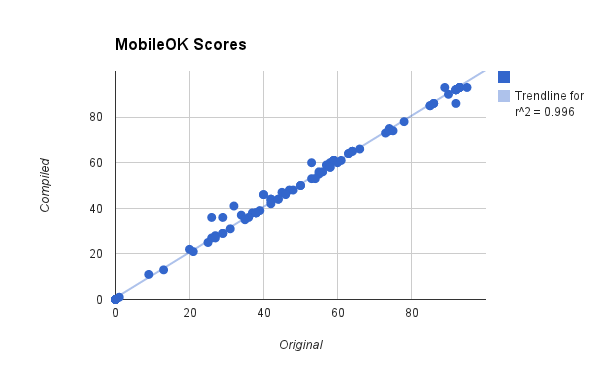
\includegraphics[scale=0.4]{mobileokrq1}
\end{figure}

\begin{figure}[h!]
    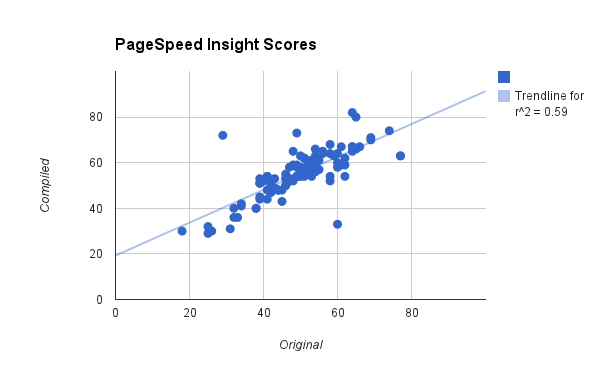
\includegraphics[scale=0.4]{pagespeedrq1}
\end{figure}

\begin{figure}[h!]
    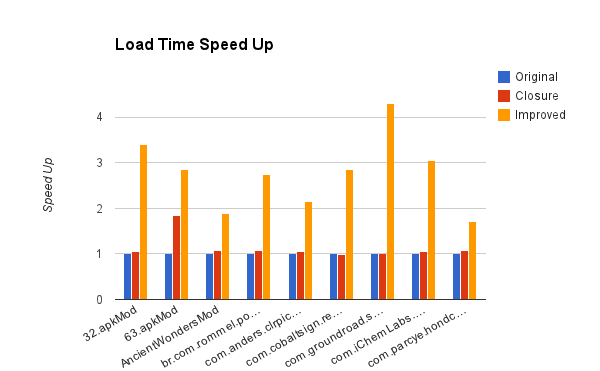
\includegraphics[scale=0.4]{loadtime}
\end{figure}

\begin{figure}[h!]
    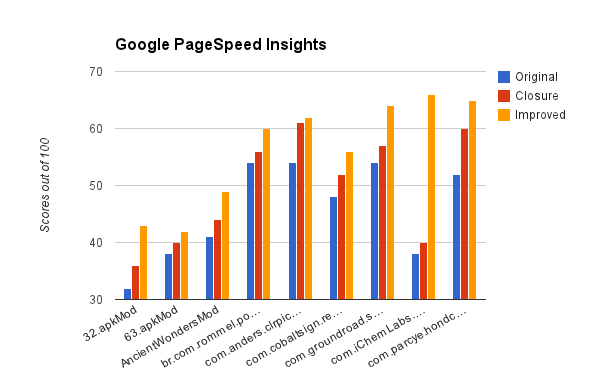
\includegraphics[scale=0.4]{pagespeeds}
\end{figure}

\section{Related Work}
% We require at least 10 references. You need to compare and contrast your work to previous work.
\subsection{Digua: Minifier and Obfuscator for Web Resources \cite{ciminiandigua}}
Ciminian and Dobre discuss their minifier tool Digua in \cite{ciminiandigua}. 
Digua is a minifier which works for CSS, HTML, and JavaScript.  
It will find correlations between these different languages to further reduce the size of these files.
The paper states that 80\% of web page loading time is attributed to loading page resources and only 20\% is from back-end computations and the reduced file size will result in much increased web page responsiveness.
This does not apply to hybrid mobile apps.
This is because the web code for the application is already stored in the device.
The method presented in the paper would only apply to applications which need to be downloaded every time the website is hit. 

\subsection{Semi-Automatic Rename Refactoring for JavaScript \cite{feldthaus2013semi}}
% cut this one?
Feldthaus and Moller discuss a method for renaming functions using a combination of static analysis and programmer input in \cite{feldthaus2013semi}.
While this does not apply directly to our project, it does bring up issues involved with renaming in JavaScript.
For instance, similarly named features of the code may be renamed when they should not be.
This will lead to a lot of errors in the code.
This is a limitation to minification methods as well, since, in order to maintain functionality, certain features such as functions cannot be renamed.

\subsection{Modern JavaScript Project Optimizers \cite{zolotareva2014modern}}
Zolotareva et. al. in \cite{zolotareva2014modern} discuss the state of the art of JavaScript optimizers.
Tools discussed included JSMin, YUI Compressor, UglifierJS, Google Closure Compiler, and KJSCompiler and their respective benefits and drawbacks.
For instance, KJSCompiler is an extension to Google Closure Compiler where the users can annotate dependencies between files.
This is a useful tool to research due to the fact that it may further reduce the size of JavaScript files and combine them into a single library.
These tools could all fit in our process to determine if old guidelines do not create improvements for hybrid applications.
With regard to scale of work for the term, we are currently considering just the Google Closure compiler.

\subsection{Characterizing and Detecting Performance Bugs for Smartphone Applications \cite{liu2014characterizing} }
This paper begins by presenting common patterns among performance bugs among popular, large scale Android applications.
Then, the paper presents PerfChecker, a static analysis tool that looks for those performance bugs (20 of which were fixed by developers).
This paper focuses on bugs relating to a native application’s local code and potentially very specific causes for those bugs, such as activating multiple features in a specific sequence.
So, the guidelines presented here do not directly address hybrid mobile applications, although the approach or results could in some cases be adapted for hybrids.
For instance, the general recommendation of recycling resources on a page instead of creating memory bloat by adding and deleting constantly can be derived from the memory bloat bug type in this paper.

\subsection{AppMobiCloud \cite{Wang:2013:AIM:2532443.2532445}}
Wang et. al. in \cite{Wang:2013:AIM:2532443.2532445} look to improve the performance of mobile web applications by partitioning computation-intensive portions of code and offloading it to servers for remote execution. 
AppMobiCloud is the tool that does this, ensuring that an app's functionality remains the same but it performs faster and saves energy on the mobile device.
The tool uses a code analyzer to find the computations to offload. 
AppMobiCloud technique of offloading computation to servers is different our technique of finding code changes that run on the device that will improve performance.
Also, although they target mobile web applications and this paper targets mobile hybrid applications, both types could likely benefit from computational offloading.
This is a potential future work because, to the best of our knowledge, this avenue has not been explored in the current literature.

\subsection{A Comparative Analysis of Cross-platform Development Approaches for Mobile Applications \cite{Xanthopoulos:2013:CAC:2490257.2490292}}
\cite{Xanthopoulos:2013:CAC:2490257.2490292} compares the use of four types of mobile applications: web, hybrid, interpreted, and generated. 
This survey of current technologies highlights that native apps provide a great experience but have a high development cost due to requiring device-specific implementations.
Hybrid and interpreted apps avoid this deployment issue because the code for these apps is written once and interpreted in the required way by the devices. 
\cite{Xanthopoulos:2013:CAC:2490257.2490292} also reports that generated apps give a great alternative to native apps but there is little support for this paradigm without commercial purchases. 
These results discuss the pros and cons of a high level design decision, where our reported code changes focus on lower level code changes and their pros and cons.

\subsection{Discovering Refactoring Opportunities in Cascading Style Sheets \cite{Mazinanian:2014:DRO:2635868.2635879}}
Mazinanian et. al. explore ways to improve CSS, primarily for maintainability in \cite{Mazinanian:2014:DRO:2635868.2635879}. 
That paper provides description of CSS duplications, refactoring improvements, ranking of those refactorings for prioritization, and preconditions for preservation of styling after refactoring.
Our paper could have suggested following what was presented in \cite{Mazinanian:2014:DRO:2635868.2635879}, but there is not a strong indication our metrics would have improved.
Their technique reduced file size by 8% which may have sped file parsing and improved loading time, but just minifying the CSS may have similar effects at a reduced cost.

\subsection{MobiTran: Tool Support for Refactoring PC Websites to Smart Phones \cite{Ma:2013:MTS:2541614.2541621}}
In \cite{Ma:2013:MTS:2541614.2541621}, Ma et. al. present MobiTran which helps developers create a smart phone ready website from a desktop website. 
Their approach highlights some differences between websites on PC and smart phones but does not address differences for hybrid applications. 
Their paper does explain how transformations of certain portions of websites may be generalized to streamline their process, but these transformations do not necessarily improve loading times or help with the other metrics highlighted in our paper. 
It may be that the touch-centric transformations improve scores on MobileOK because of its recommendation of using links on entire images instead of click boxes that do not cover the entire image.

\subsection{How Do Code Refactorings Affect Energy Usage? \cite{Sahin:2014:CRA:2652524.2652538}}
In \cite{Sahin:2014:CRA:2652524.2652538}, Sahin et. al. explore the energy consumption of programs after refactorings are performed. 
It focuses on refactorings in Java programs on PCs, not hybrid applications on mobile devices. 
By focusing on energy consumption, \cite{Sahin:2014:CRA:2652524.2652538} considers one of the many elements that impact user experience. 
We focus on metrics that affect the user's perceptions in the moment, such as loading times or render blocking as reported by PageSpeed Insights.

\subsection{High Performance Web Sites\cite{souders2008high}}
The paper discussed the importance of front-end performance.
It also lists best practices and shows why they are important.
\vspace{-1.0em}
\begin{enumerate}\itemsep1pt \parskip0pt \parsep0pt
	\item Make fewer HTTP requests
	\item Use a content delivery network
	\item Add an Expires header
	\item Gzip components
	\item Put stylesheets at the top
	\item Put scripts at the bottom
	\item Avoid CSS expressions
	\item Make JavaScript and CSS external
	\item Reduce DNS lookups
	\item Minify JavaScript
	\item Avoid redirects
	\item Remove duplicate scripts
	\item Configure ETags
	\item Make Ajax cacheable
\end{enumerate}

\section{Project Experience}
\subsection{Corpus}
We had a rough time obtaining a corpus. We first started by scanning the internet and Github for open source phonegap applications, and found small applications that would not have been great for our research. Many of the repositories were just examples, and tutorials. The phonegap website had a list of 720 phonegap applications with links to their apks. Apks were not useful to use because they were packaged up and didn't have the source code. So we decided to pull the list of phonegap applications and associated developers. We used this list of search for open source projects on github, but many repositories were links to download the apks, small example libraries, or applications with incomplete source. 

\section{Conclusion}
% This is a brief summary, but also contains the most surprising findings, implications, directions for future research.
By combining the described changes into an automated refactoring tool, these improvements could be made in many applications.

\section{Acknowledgments}
This paper was possible because of Dr. Danny Dig; Aharon Abadi of IBM; the makers of Google Closure Compiler, MobileOK, PageSpeed Insights; and the writers of all the apps we used for the experiment.

\bibliographystyle{plain}
\bibliography{sigproc-sp}

\end{document}
